% Copyright 2004 by Till Tantau <tantau@users.sourceforge.net>.
%
% In principle, this file can be redistributed and/or modified under
% the terms of the GNU Public License, version 2.
%
% However, this file is supposed to be a template to be modified
% for your own needs. For this reason, if you use this file as a
% template and not specifically distribute it as part of a another
% package/program, I grant the extra permission to freely copy and
% modify this file as you see fit and even to delete this copyright
% notice. 

\documentclass[aspectratio=169]{beamer}
%\documentclass{beamer}

\setbeamersize{text margin left=5mm, text margin right=5mm}


\defbeamertemplate{headline}{my header}{%
\vskip1pt%
\makebox[0pt][l]{\,\insertshortauthor}%
\hspace*{\fill}\insertshorttitle/\insertshortsubtitle\hspace*{\fill}%
\llap{\insertpagenumber/\insertpresentationendpage\,}
}
\setbeamertemplate{headline}[my header]

\let\olditem\item
\renewcommand{\item}{\setlength{\itemsep}{\fill}\olditem}

\usepackage{soul}
\usepackage{tkz-euclide}
\usetikzlibrary{calc}
\usepackage[]{algorithm2e}
\usepackage{changepage}
\usepackage{amssymb}
\usepackage{xcolor}
\usepackage{mathtools}
\usepackage{tcolorbox}
\usepackage{tikz}
\usepackage{tikz-3dplot}
\usepackage[export]{adjustbox}
\usepackage{tabu}

% \usepackage[math]{cellspace}
% \cellspacetoplimit 4pt
% \cellspacebottomlimit 4pt
%\usetikzlibrary{arrows.meta}

%\setbeamertemplate{itemize items}{-}

%\usepackage{helvet}
\usefonttheme{professionalfonts} % using non standard fonts for beamer
%\usefonttheme{serif} % default family is serif
%\usepackage{fontspec}
%\setmainfont{Liberation Serif}

% There are many different themes available for Beamer. A comprehensive
% list with examples is given here:
% http://deic.uab.es/~iblanes/beamer_gallery/index_by_theme.html
% You can uncomment the themes below if you would like to use a different
% one:
%\usetheme{AnnArbor}
%\usetheme{Antibes}
%\usetheme{Bergen}
%\usetheme{Berkeley}
%\usetheme{Berlin}
%\usetheme{Boadilla}
%\usetheme{boxes}
%\usetheme{CambridgeUS}
%\usetheme{Copenhagen}
%\usetheme{Darmstadt}
%\usetheme{default}
%\usetheme{Frankfurt}
%\usetheme{Goettingen}
%\usetheme{Hannover}
%\usetheme{Ilmenau}
%\usetheme{JuanLesPins}
%\usetheme{Luebeck}
%\usetheme{Madrid}
%\usetheme{Malmoe}
%\usetheme{Marburg}
%\usetheme{Montpellier}
%\usetheme{PaloAlto}
%\usetheme{Pittsburgh}
%\usetheme{Rochester}
%\usetheme{Singapore}
%\usetheme{Szeged}
%\usetheme{Warsaw}


\def\mf{\ensuremath\mathbf}
\def\mb{\ensuremath\mathbb}
\def\mc{\ensuremath\mathcal}
\def\lp{\ensuremath\left(}
\def\rp{\ensuremath\right)}
\def\lv{\ensuremath\left\lvert}
\def\rv{\ensuremath\right\rvert}
\def\lV{\ensuremath\left\lVert}
\def\rV{\ensuremath\right\rVert}
\def\lc{\ensuremath\left\{}
\def\rc{\ensuremath\right\}}
\def\ls{\ensuremath\left[}
\def\rs{\ensuremath\right]}
\def\bmx{\ensuremath\begin{bmatrix*}[r]}
\def\emx{\ensuremath\end{bmatrix*}}
\def\bmxc{\ensuremath\begin{bmatrix*}[c]}
\def\t{\lp t\rp}
\def\k{\ls k\rs}


\newcommand{\demoex}[2]{\onslide<#1->\begin{color}{black!60} #2 \end{color}}
\newcommand{\demoexc}[3]{\onslide<#1->\begin{color}{#2} #3 \end{color}}
\newcommand{\anim}[3]{\onslide<#1->{\begin{color}{#2!60} #3 \end{color}}}
\newcommand{\ct}[1]{\lp #1\rp}
\newcommand{\dt}[1]{\ls #1\rs}
\newcommand{\cols}[2]{\begin{columns}[#1] #2 \end{columns}}
\newcommand{\col}[2]{\begin{column}{#1} #2 \end{column}}

\newcommand{\xdownarrow}[1]{%
  {\left\downarrow\vbox to #1{}\right.\kern-\nulldelimiterspace}
}

\title{Introduction to Digital Signal Processing}

% A subtitle is optional and this may be deleted
\subtitle{Z-transform}

\author{Sivakumar Balasubramanian}
% - Give the names in the same order as the appear in the paper.
% - Use the \inst{?} command only if the authors have different
%   affiliation.

\institute[Christian Medical College] % (optional, but mostly needed)
{
  \inst{}%
  Department of Bioengineering\\
  Christian Medical College, Bagayam\\
  Vellore 632002
}
% - Use the \inst command only if there are several affiliations.
% - Keep it simple, no one is interested in your street address.

\date{}
% - Either use conference name or its abbreviation.
% - Not really informative to the audience, more for people (including
%   yourself) who are reading the slides online

\subject{Lecture slides on Introduction to DSP}
% This is only inserted into the PDF information catalog. Can be left
% out. 

% If you have a file called "university-logo-filename.xxx", where xxx
% is a graphic format that can be processed by latex or pdflatex,
% resp., then you can add a logo as follows:

% \pgfdeclareimage[height=0.5cm]{university-logo}{university-logo-filename}
% \logo{\pgfuseimage{university-logo}}

% Delete this, if you do not want the table of contents to pop up at
% the beginning of each subsection:
\AtBeginSubsection[]
{
  \begin{frame}<beamer>{Outline}
    \tableofcontents[currentsection,currentsubsection]
  \end{frame}
}

% Let's get started
\begin{document}

\begin{frame}
  \titlepage
\end{frame}


\begin{frame}[t]{Z transform}
\begin{itemize}
  \item Exponential signals are \textit{eigenfucntiopns} of LTI systems.
  \[  z^n \longrightarrow H\lp z \rp z^n \]
  $H(z)$ is the eigenvalue corresponding to the eigenfunction $z^n$.

  \item If $x[n] = \sum_{k} \alpha_k z_k^n$, then $y[n] = \sum_{k} \alpha_k H\lp z_k \rp z_k^n$.
  \[ \begin{split}
      \lp \alpha_k \rp_{k \in \mb{Z}} & \longrightarrow \text{Representation of } x[n] \text{ using } z_k^n \\
      \lp H\lp z_k \rp \alpha_k \rp_{k \in \mb{Z}} & \longrightarrow \text{Representation of } x[n] \text{ using } z_k^n \\
      \end{split} \]

  \item The z-transoform allows us to find the representation of any disctet-time signal $x[n]$ in terms of the set of complex exponentials $\{ z^n \}_{z \in \mb{C}}$ 
\end{itemize}
\end{frame}


\begin{frame}[t]{z transform}
The z-transform of a discrete time signal $x[n]$ is defined as the following power seris,
\[ X\lp z \rp \triangleq \sum_{n=-\infty}^{\infty} x[n] z^{-n} = \mc{Z}\lp x[n] \rp\]
\[ x[n] \xleftrightarrow{\mc{Z}} X\lp z \rp  \]
where, $z \in \mb{C}$.

\begin{itemize}
  \item The values of $z$ for which the above summation covnerges is called the \textit{region of conergence} of $X(z)$.
\end{itemize}
\end{frame}


\begin{frame}[t]{z transform}
z-transform of some signals.
\begin{enumerate}
  \item $\delta[n]$
  \item $\delta[n-k]$
  \item $\delta[n+k]$
  \item $\sum_{k=0}^{5} \alpha_k \delta[n - k]$
  \item $1[n]$
  \item $a^k \cdot 1[n]$
  \item $-a^{k} \cdot 1[-n-1]$
\end{enumerate}
\end{frame}


\begin{frame}[t]
  \frametitle{z-transform and ROCs}
  \begin{center}
  \begin{figure}
  \centering
  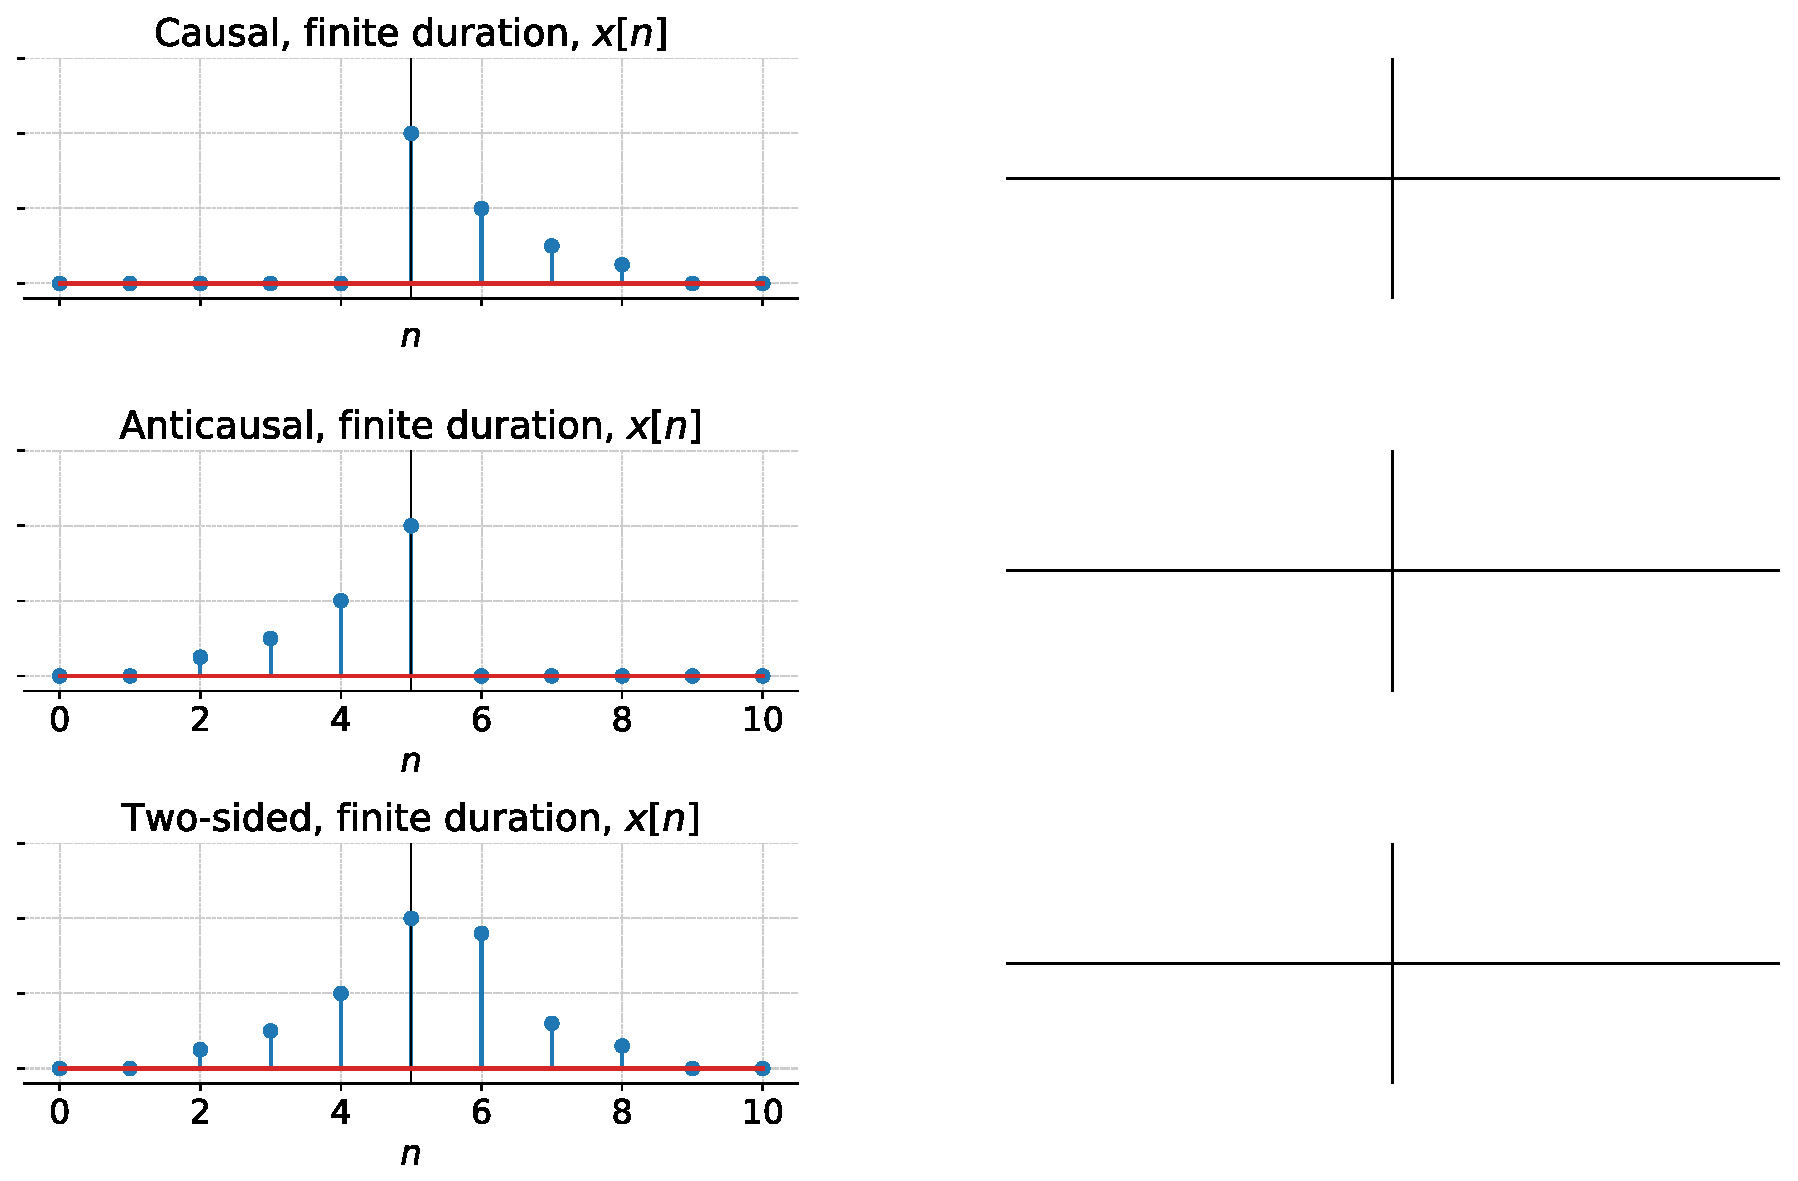
\includegraphics[width=0.7\textwidth, left]{img/ztrans-finite-dur.eps}
  \end{figure}
  \end{center}
\end{frame}


\begin{frame}[t]
  \frametitle{z-transform and ROCs}
  \begin{center}
  \begin{figure}
  \centering
  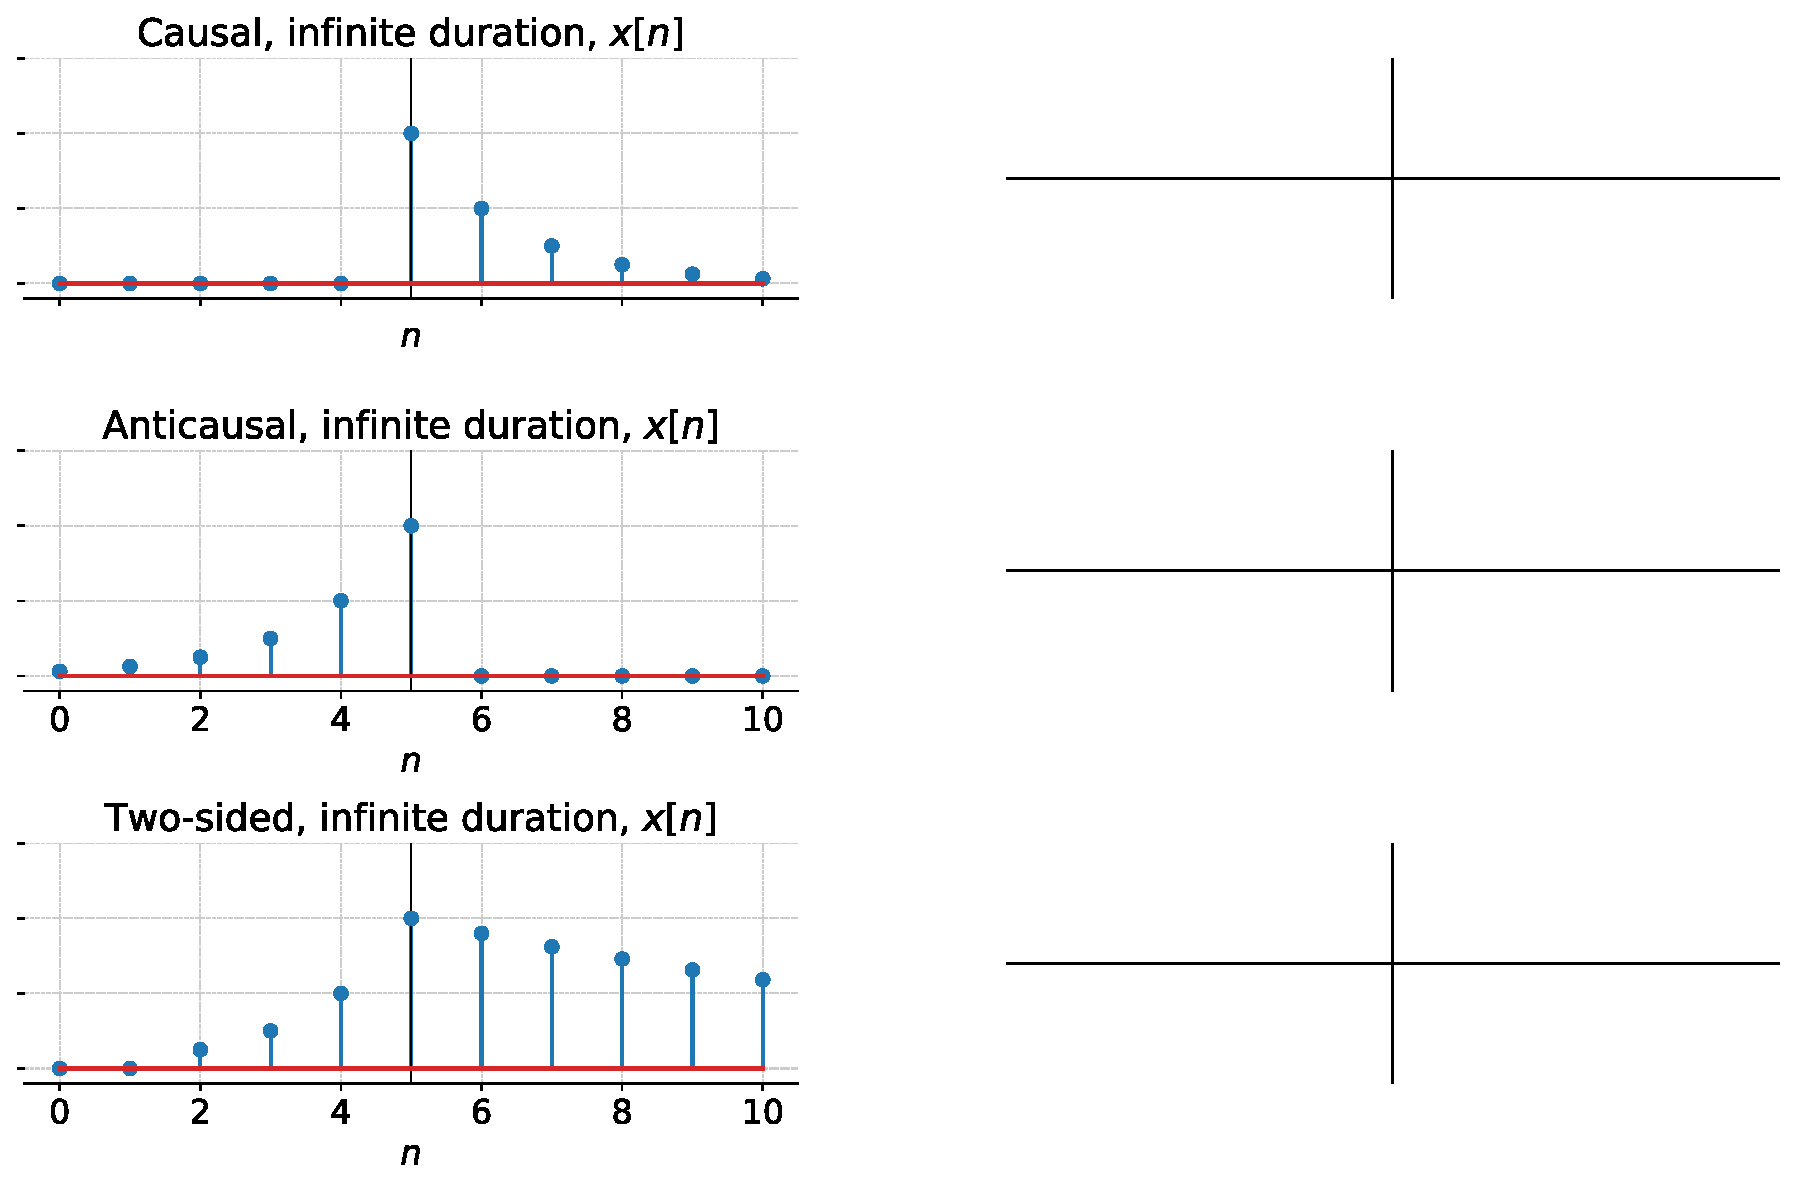
\includegraphics[width=0.7\textwidth, left]{img/ztrans-infinite-dur.eps}
  \end{figure}
  \end{center}
\end{frame}


\begin{frame}[t]
  \frametitle{Properties of the z-transform}
  \begin{itemize}
      \item Linearity
      \item Time-shifting
      \item Convolution in time
      \item Initital value theorem
    \end{itemize}  
\end{frame}

\begin{frame}[t]
  \frametitle{Unilateral z-transform}

  z-transform of causal signals of the form $x[n]\cdot 1[n]$.

  \[ X(z) = \sum_{n=0}^{\infty} x[n] z^{-n} \]
  
  This is useful when analysing linear difference equations.

  When the time domain signal $x[n]$ is delayed by a sample, such that the signal is $x[n-1] \cdot 1[n]$, then we have
  \[ x[n] \cdot 1[n] \xleftrightarrow{\mc{Z}_{ul}} X(z) \implies x[n-1] \cdot 1[n] \xleftrightarrow{\mc{Z}_{ul}} z^{-1} X\lp z \rp + x[-1] \] 
\end{frame}

\begin{frame}[t]
  \frametitle{Transfer function of an LTI system}

  The z-transform of the impulse response $h[n]$ is defined as the transfer function of a discrete-time LTI system.
  \[ H\lp z \rp = \sum_{n=-\infty}^{\infty} h[n] z^{-n} \]

  When the system is causal, then $H\lp z \rp = \sum_{n=0}^{\infty} h[n] z^{-n}$.

  The z-transforms of the input $x[n]$ and $y[n]$ are related to each other through the transfer function, 
  \[ Y(z) = H(z) \cdot X(z) \]
\end{frame}

\begin{frame}[t]
  \frametitle{Rational z-transforms}
  \begin{itemize}
    \item In practice, we often come across rational polynomial of $z$.
    \item Consider a LTI system described by the following different equation,
    \[ y[n] + a_1 y[n-1] + a_2 y[n-2] + \cdot + a_Ny[n - N] = b_0x[n] + b_1 x[n-1] + \cdots + b_M x[n - M] \] 
    We are interested in sovling this equation from time $n = 0$ for an input of the form $x[n]\cdot 1[n]$. Taking the unilateral z-transform on both sides,
    \[ \begin{split}
        y[n] \xleftrightarrow{\mc{Z}_{ul}} \,\, & \,\, Y(z) \\
        y[n-1] \xleftrightarrow{\mc{Z}_{ul}} \,\, & \,\, z^{-1}Y(z) + y[-1] \\
        y[n-2] \xleftrightarrow{\mc{Z}_{ul}} \,\, & \,\, z^{-2}Y(z) + z^{-1}y[-1] + y[-2] \\
        \vdots & \\
        y[n-N] \xleftrightarrow{\mc{Z}_{ul}} \,\, & \,\, z^{-N}Y(z) + z^{-(N-1)}y[-1] + z^{-(N-2)}y[-2] + \cdots + y[-N]
        \end{split} 
        \]
  \end{itemize}
\end{frame}

% \begin{frame}[t]
%   \frametitle{Fourier transform of a Modulated Impulse train}
%   \begin{figure}
%   \centering
%   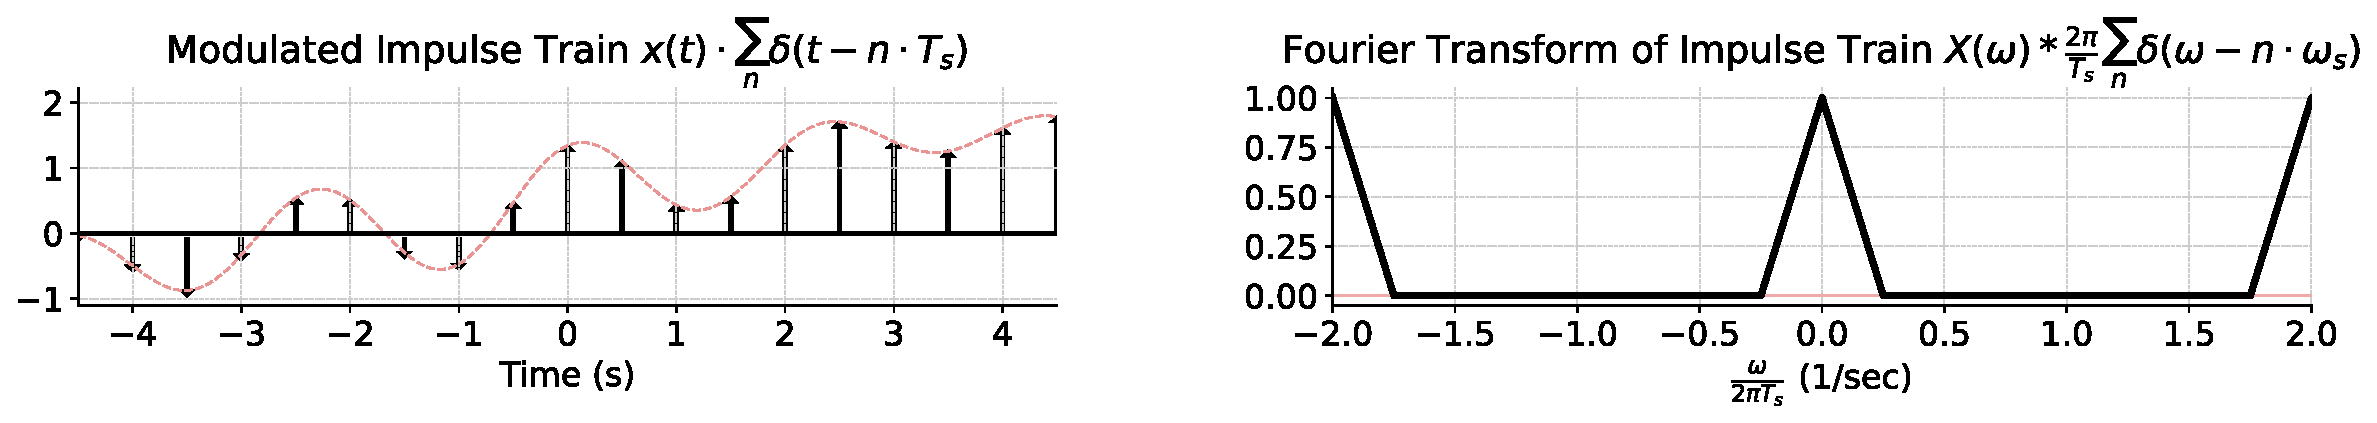
\includegraphics[width=1\textwidth, left]{img/sampling2.eps}
%   \end{figure}
% \end{frame}


% \begin{frame}[t]
%   \frametitle{Sampling at the Nyquist rate}
%   \begin{figure}
%   \centering
%   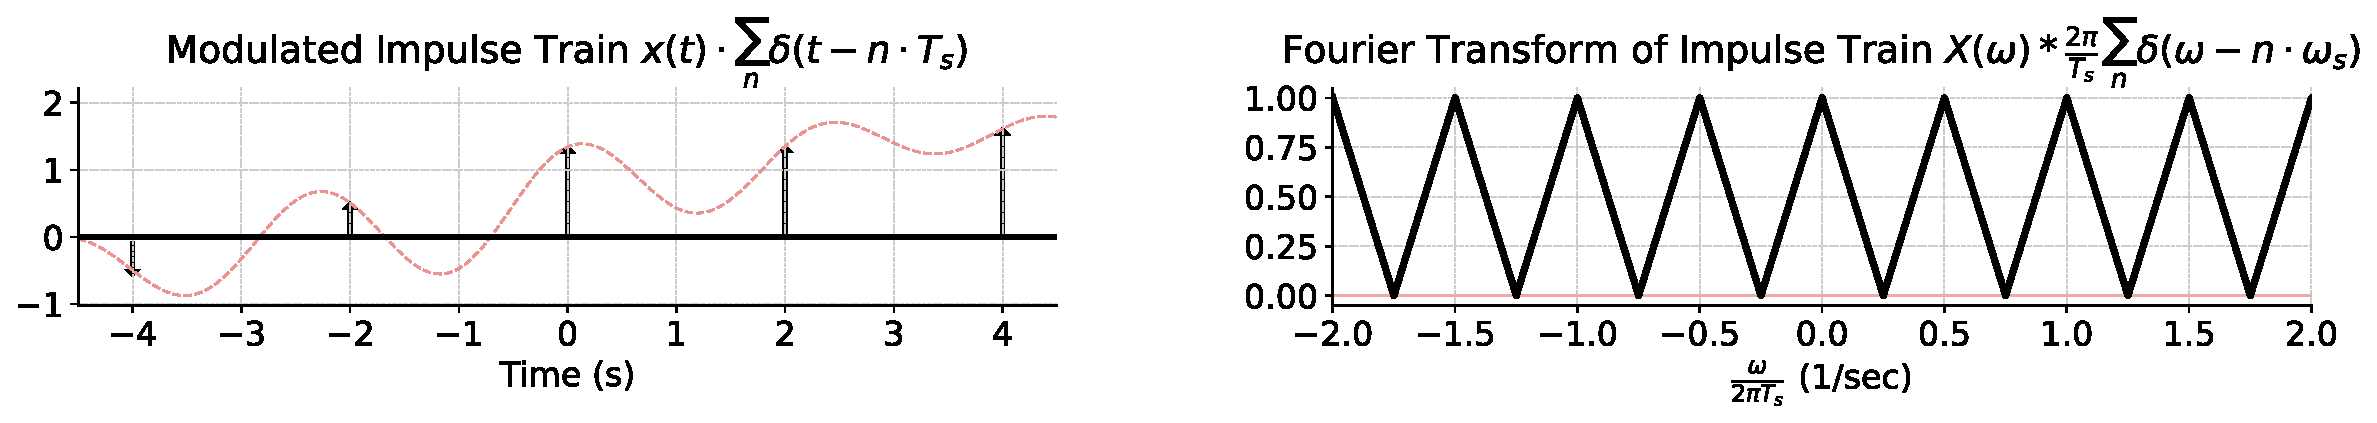
\includegraphics[width=1\textwidth, left]{img/sampling4.eps}
%   \end{figure}
% \end{frame}


% \begin{frame}[t]
%   \frametitle{What happens when the signal is not bandlimited?}
%   \begin{figure}
%   \centering
%   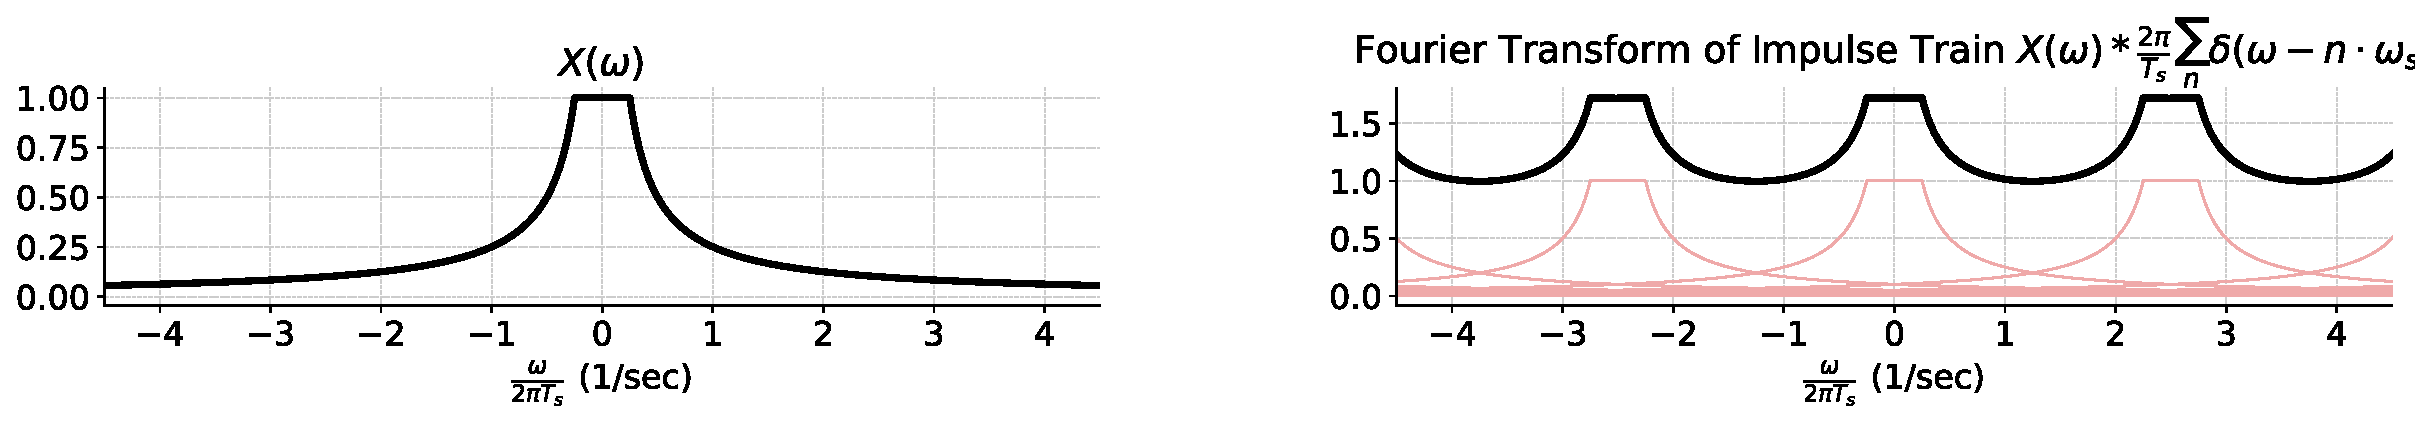
\includegraphics[width=1\textwidth, left]{img/sampling-nbl.eps}
%   \end{figure}

%   \begin{figure}
%   \centering
%   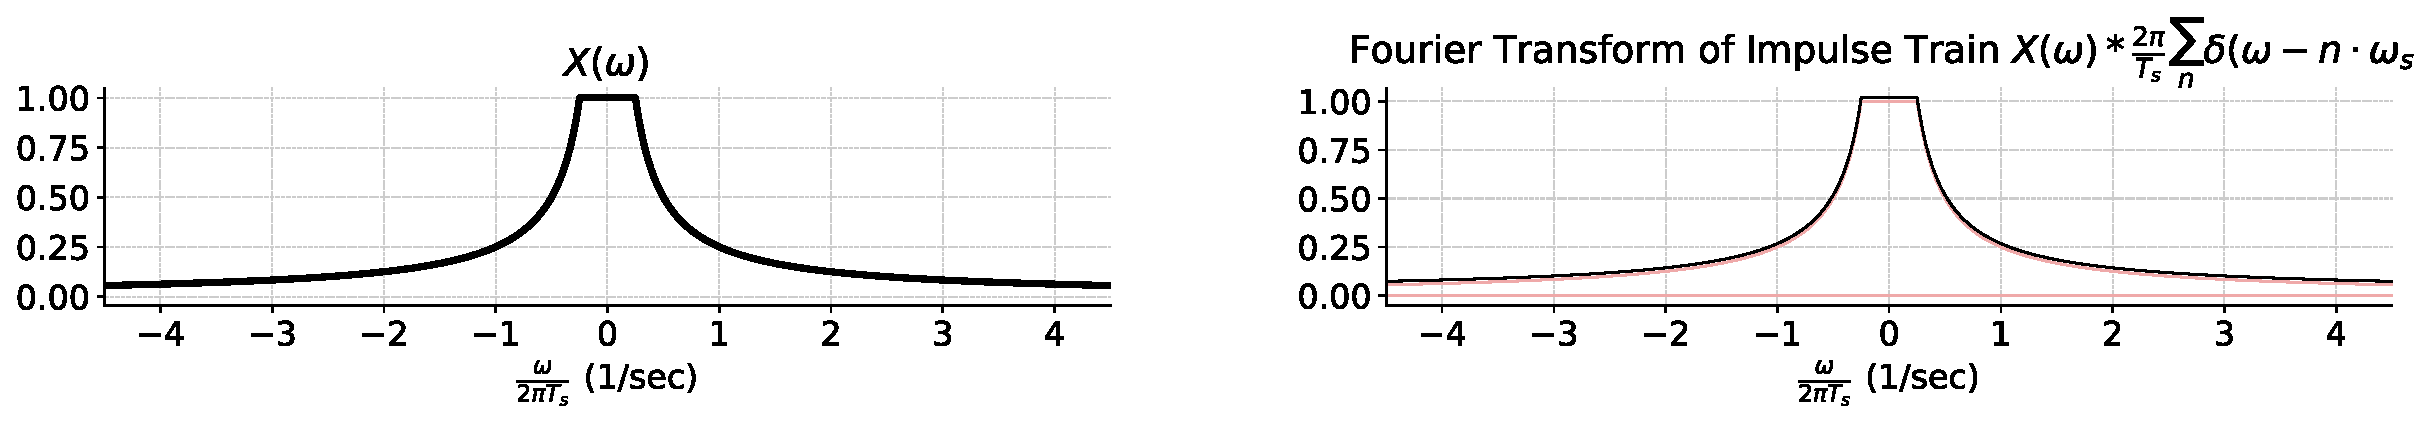
\includegraphics[width=1\textwidth, left]{img/sampling-nbl-high.eps}
%   \end{figure}
% \end{frame}


\end{document}